% =====================================================================
%  chunks/appc.tex —— 原书 p.292–298（PDF 299–305）
%  附录：3 维流形与纽结拓扑学的新进展
%  §4 3 维流形的新拓扑不变量与拓扑量子场论（续）
% =====================================================================

% [原文 p.292]
这里 $k$ 是整数，其依据是「耦合常数的拓扑量子化」（由本书作者于 1981 年对多值泛函表述，Deser--Jackiw--Templeton 在 Chern--Simons 作用量的特殊情形下于 1982 年给出，Witten 于 1983 年给出），而这又是「Feynman 振幅」$\exp\{ikS\}$ 应当为单值这一要求的推论。注意 Chern--Simons 作用量有如下局部形式：
\[
S(A)=\Tr\Bigl(\partial_iA_i-\partial_jA_j+\frac23A^3\Bigr).
\]

% [Tutor Note: 原书把 Chern--Simons 作用量写成这个「局部形式」，但式中下标 $i,j$ 并未按 Einstein 约定缩并，$\partial_iA_i$ 也不是坐标不变的写法；其标准形式是 $S(A)=\int_M\Tr\bigl(A\wedge dA+\frac23A\wedge A\wedge A\bigr)$。此处照录原书，读者按标准形式理解即可。]

利用 3 维流形沿某曲面的 Heegaard 分解，Witten 发展出拓扑量子场论的一种漂亮的「Hamilton 化」途径，使他能把定义与计算量 $Z(M^3)$ 的问题归结为该曲面上 2 维共形场论的某些问题。Axelrod 与 Singer（以及在特殊情形下由 Kontzevich）关于 $Z(M^3)$ 在变量 $\frac1k\to\infty$ 下的扰动级数，给出了一些有趣的拓扑量；但这些量的性质与可能的应用迄今尚未被研究。

给出这一不变量的精确、严格、非微扰且纯拓扑的定义这一问题，由 Reshetikhin 与 Turaev 解决。这类不变量的理论又由若干人进一步发展，其中包括 Viro、Lawrence 与 Lickorish。下面我们将描述其中一些不变量，按 Lickorish 1980 年代末的工作来叙述。（我们对这项工作的叙述主要取自 Kauffman 的书《Knots and Physics》。）

任何 3 维流形 $M_L^3$ 都可以通过在 $S^3$ 中沿某个适当的链环或纽结 $L$ 作手术而得到。这种实现 3 维流形的方式，曾被 Lickorish、Zieschang 与本书作者在 1960 年代初用于在任意闭 3 维流形上构造非奇异的 2 维叶状结构：从 $S^3$ 的 Reeb 纤维化出发，沿某个适当的横截纽结或链环作「管化」（tubulization）运算，即沿 $S^1\times D^2\subset S^3$ 中某个适当的闭辫来作。看来 Dehn 早已知道可以通过沿 $S^3$ 中的纽结或链环作手术得到任意 3 维流形；而化归到闭辫则肯定应归于 Alexander（见上文）。1980 年代的某个时候，Kirby 指出这一构造中的自由度可以用两个标准的基本运算来刻画，这两个运算出现在 Smale 与 Wallace 证明 $n$ 维 Poincaré 猜想（$n>4$）时所用的多维手术理论之中。所论的两个运算如下（现在还假定链环带有「框」，见下文）：

\begin{enumerate}
\item 第一个 Kirby 运算是给链环添加一个不打结的分支，用一堵「墙」$\R^2\subset\R^3$ 把它与原链环隔开，并使其框的环绕系数为 $\pm1$（见下文）。

% [原文 p.293]

\item 第二个 Kirby 运算如下：取两个分支 $L_i,L_j$，并把其中之一（$L_i$）的平行移位记为 $L_i^1$。用一条 Jordan 弧把 $L_i$ 与 $L_j$ 连接起来，该弧带有与 $L_i$、$L_j$ 上的法标架相容的法标架，且不与其余分支相交。沿这条带框的弧作 $L_i$ 与 $L_j$ 的「连通和」$\bar L_j$，这类似于带框手术理论中的「连通和」构造（例如按 Pontryagin 的方案计算 $\pi_3(S^2)$ 时所用者）。最后，把这一对 $L_i,L_j$ 换成新的一对 $L_i^1,\bar L_j$（其余分支保持不变）。
\end{enumerate}

\begin{figure}[htbp]
\centering
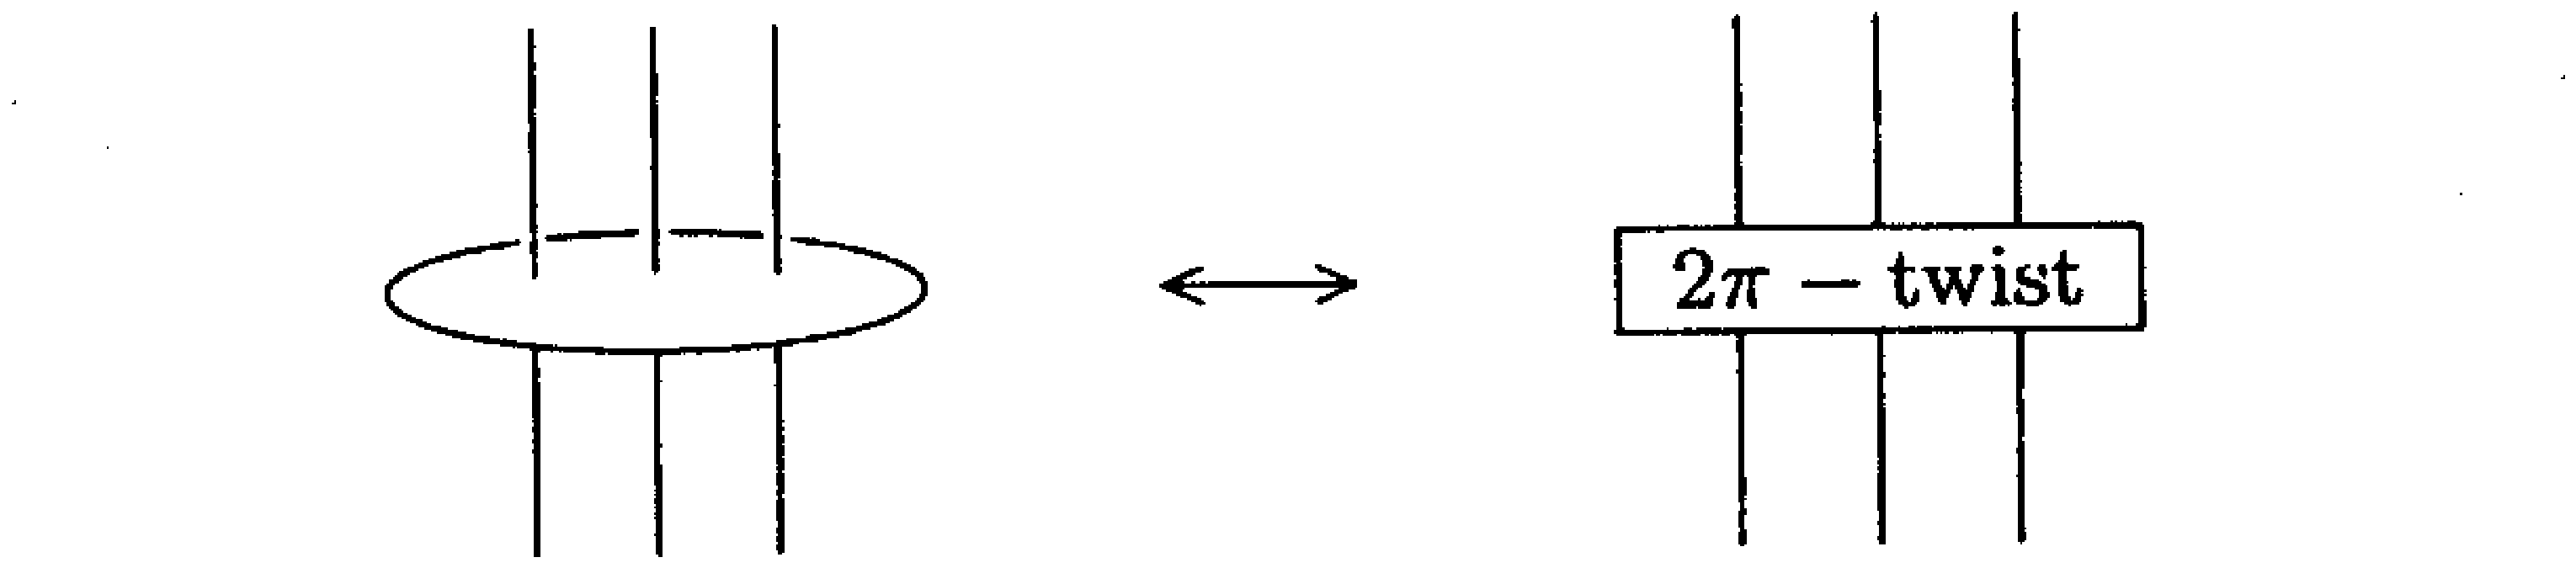
\includegraphics[width=0.80\textwidth]{figures/figA13.png}
\figtitle{A.13}{$2\pi$ 扭转}
\end{figure}

（代替第二个运算，研究 3 维流形的学者往往更喜欢用两个运算的某种组合。例如，若链环具有如下形状：一个环绕系数为 $\pm1$ 的不打结带框圆周（见下文）围住一个圆盘，另有若干分支都横截地与这个圆盘相交；那么就移去这个不打结的分支，并对其余分支施以「$2\pi$ 扭转」（见图 A.13）。）如上所述，在目前的语境中，所给的纽结或链环都假定自带一个框（即 $\R^3$ 中的单位法向量场）。这种框的完全的拓扑不变量，由原曲线（分支）$S^1$ 与它沿法向量场方向作小距离移位所得曲线之间的环绕系数给出。所谓\emph{标准法标架}就是使这个环绕系数为零的框：$\{S^1,S_1^1\}=0$。沿 3 维流形 $M^3$ 中的一条闭 Jordan 曲线 $S^1$（其法丛平凡，$T(S^1)=S^1\times D^2\subset M^3$）作手术，完全由该曲线的一个框的环绕系数所决定：在新流形 $M_L^3$ 中，移位 $S_1^1$ 应当是零伦的（若沿链环作手术，则对链环的每个分支都同样处理）。

对一个带框链环 $L$，有一个\emph{环绕矩阵}，即一个对称的 $n\times n$ 矩阵，其中 $n$ 是分支数。链环的\emph{指标} $i(L)$ 则定义为该环绕矩阵对角化后严格负的元素的个数。

\emph{黑板框}是链环 $L$ 的平面图的法向量场，由某个通有的平面投影得到。把纽结或链环 $L$ 沿垂直于投影平面的方向作小距离移位，便得到一条平行纽结或平行链环。若 $D$ 是链环的任一图，我们将把同一个图 $D$（其 $n$ 个分支按某种次序编号为 $1,2,\dots,n$）标上整数 $i_1,\dots,i_n$，就表示一个新的链环：其中第 $q$ 个分支（标号为 $i_q$ 者）换成 $i_q$ 条彼此靠得很近、与该分支平行的分支。于是这个新链环总共有 $i_1+\dots+i_n$ 个分支。

% [原文 p.294]

对每个固定的正整数 $r$，记 $I_r=\{0,1,\dots,r-2\}$，并用 $c$ 表示从链环的分支集合（编号 $1,2,\dots,n$）到 $I_r$ 的任一函数。给定任意一组数 $\lambda_0,\lambda_1,\dots,\lambda_{r-2}$，我们按下式定义一个数 $\langle\langle L\rangle\rangle$（其中 $L$ 指所论的链环）：
\[
\langle\langle L\rangle\rangle=\sum_c\lambda_{c(1)}\times\cdots\times\lambda_{c(n)}S_{D_L}(A,A^{-1};\delta);
\]
这里求和遍历所有这样的函数 $c$，而 $\delta=-A^2-A^{-2}$（如 Kauffman 构造 Jones 多项式时那样——见前文），$D_L$ 表示链环 $L$ 的图。

公式
\[
TR(M_L^3)=\delta^{-i(L)}\langle\langle L\rangle\rangle
\]
便给出 3 维流形 $M_L^3$ 的一个拓扑不变量（即 $TR$ 或 \emph{Turaev--Reshetikhin 不变量}），条件是 $r\ge3$、$A=\exp\{i\pi/2r\}$，且诸 $\lambda_q$ 满足超定的线性方程组
\[
\delta^j=\sum_{i=0}^{i=r-2}\lambda_iT_{i+j},\qquad j\ge0,
\]
其中 $T_j$（$j\in\Z$）表示由「恰有一个交叉的基本图」的 $j$ 个互不相交的平行拷贝所构成的图 $D_j$ 决定的量 $S_{D_j}(A,A^{-1};\delta)$（见图 A.14）。尽管这一不变量具有相当的内在意义，它迄今尚未在解决任何拓扑问题中得到应用。

\begin{figure}[htbp]
\centering
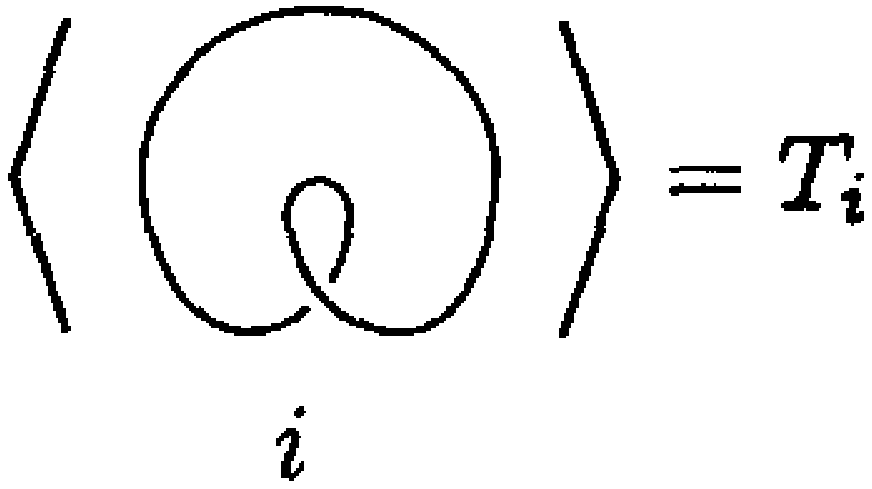
\includegraphics[width=0.42\textwidth]{figures/figA14.png}
\figtitle{A.14}{基本图及其平行拷贝}
\end{figure}

「拓扑量子场论」（TQFT）这一重要概念是近年来出现的，其背景是人们开始认识到：TQFT 所表示的并不只是用泛函积分或更严格的组合途径来构造纽结与流形的某些拓扑不变量。下面我们叙述 TQFT 的一套公理系统，它由 Segal 与 Atiyah 提出。（这套系统或可看作与同调论中著名的 Eilenberg--Steenrod 公理系统相类似，后者在与 $K$-理论、复配边理论等同调论的推广相关联时特别有用。）

% [原文 p.295]

一个 $n$ 维 TQFT 被公设为：一个由闭的定向 $(n-1)$ 维流形 $V$ 构成的范畴，每个 $V$ 都配以一个 Hilbert 空间 $H_V$（通常是有限维的）。态射则对应于定向 $n$ 维流形 $W$，其边界 $V$ 分成两部分（「内部」与「外部」）：
\[
\partial W=V=V_1\cup V_2,
\]
其中 $V_1,V_2$ 带有诱导定向。任何这样的配边 $W$ 决定一个线性映射
\[
f_W:H_{V_1}\to H_{\bar V_2},
\]
（横线表示相反的定向），它可看作 $H_{V_1\cup V_2}$ 的一个元素：
\[
f_W\in H_{V_1\cup V_2}=H_{V_1}\otimes H_{\bar V_2}^*,
\]
依据是公理
\[
H_V=H_{\bar V}^*;
\]
（这里星号表示伴随空间。）显然，对于带有自然定向的柱体，映射 $f_W$ 就是恒等映射。于是，对任何以 $V$ 为边界的流形 $W$，态射由元素 $f_W\in H_V$ 所决定。

若流形 $V$ 恰好是两个流形 $W_1,W_2$ 的边界，则得到两个相应的元素
\[
f_{W_1},f_{W_2}\in H_V.
\]
于是数 $\langle f_{W_1},f_{W_2}\rangle$ 是闭流形 $W_1\cup W_2$ 的一个拓扑不变量。

在古典拓扑学中，这样的不变量只有两个例子，即偶数维流形的 Euler 示性数，以及维数为 $4k$ 的带边流形的符号差；Rohlin 与本书作者在 1960 年代中期证明的「可加性引理」表明，后一个例子满足这套公理系统。在这些例子中，空间 $H_V$ 全是一维的，而态射不过就是乘以 $\exp(\alpha\tau(W))$，其中 $\tau$ 是符号差（在较简单的情形下则是 Euler 示性数）。然而现在我们已有很多新例子，其中空间 $H_V$ 的维数超过 1；它们代表高度非平凡的 TQFT，并给出上述不变量。

当 $n=2$ 时，任何配边都可以通过迭代基本的「裤子」而得到，即边界由三个圆周 $V_1,V_2,\bar V_3$ 构成的 2 维流形，其上可定义 Morse 函数，恰有一个临界点，并且在边界的两部分 $V_1\cup V_2$ 与 $\bar V_3$ 上分别取常值。作为相应 TQFT 中的态射，这个曲面在圆周 $V=S^1$ 的空间 $H_V$ 上决定一个张量 $C_{jk}^i$；事实上它的分量恰是某个「Frobenius 代数」的结构常数，后者即带有单位元、并带有数量积 $\eta_{ij}=(\ ,\ )$、满足 $\langle fg,h\rangle=\langle f,gh\rangle$ 的交换结合代数。

% [Tutor Note: TQFT 的这套「公理系统」把 $n$ 维配边范畴函子化：$(n-1)$ 维闭流形 $V\mapsto$ Hilbert 空间 $H_V$，$n$ 维配边 $W\mapsto$ 线性映射 $f_W$。公理 $H_V=H_{\bar V}^*$ 使「把 $W$ 看成 $H_V$ 的元素」与「把 $W$ 看成映射」两种读法一致；闭流形 $W_1\cup W_2$ 之所以配上一个数 $\langle f_{W_1},f_{W_2}\rangle$，正是一般 TQFT 给出数值不变量的机制。]

% [原文 p.296]

数量积 $\eta_{ij}$ 对应于边界圆周取相同定向的柱体 $S^1\times I$。

这一构造导致「关联函数」（或 TQFT 中场的乘积的真空期望，按定义它们都是常数）的取值可如下描述。设 $\{e_i\}$ 是相应 Frobenius 代数的一组基，则可导出如下性质：

(a) 一对点的 $0$-圈关联函数等于 $\eta_{ij}$；

(b) 三元组的 $0$-圈关联函数等于
\[
C_{ijk}=\eta_{is}C_{jk}^s;
\]

(c) 任何 $0$-圈关联函数都可表成
\[
\langle e_ie_j\dots e_k,1\rangle;
\]

(d) 任何 $k$-圈关联函数都可表成
\[
\langle e_ie_j\dots e_k,H^k\rangle,
\]
其中 $H^k=\eta^{ij}e_ie_j$ 是所论的 Frobenius 代数中相应的元素。

在最有趣的情形中，人们有一族这样的理论（即一族 Frobenius 代数），它们依赖于若干参数；此时这类族的「公理化」就变得非常重要。（Witten、Dijgraaf 与 Verlinde 兄弟提出了一套合适的公理系统。）应当注意，参数空间满足某些「孤子型无色散可积族」或「流体力学型族」（按 Dubrovin 与本书作者的意义，其中涉及由参数空间上某个平坦度量决定的 Hamilton 形式）。
% [Tutor Note: 原书 p.296 把 Dijkgraaf 拼作 "Dijgraaf"（p.297 与 p.296 末段亦如此）；正文三处均照录原书拼法，读者按 Dijkgraaf 理解即可。]

\begin{remark}{}
有一些在审美上非常令人愉快的例子：空间 $H_V$（$V=S_1$）恰好成为某些 Calaby--Yau 流形上同调环的偶部，而相应的 Frobenius 代数对应于该上同调环的某些「量子形变」。这类情形的严格处理（至少部分地）已由 Yau、Kontzevich、Manin、Tian、Ruan、Piunikhin、Givental、Salamon、MacDuff 等人给出，所用技巧来自辛拓扑以及代数几何与代数拓扑。
\end{remark}

% [Tutor Note: 原书把 Calabi--Yau 拼作 Calaby--Yau（本附录 p.274 处亦如此），此处照录。又本段写作 $V=S_1$，把上标 $1$ 误排成下标；因前文一直写 $V=S^1$、$H_V$，读者按 $S^1$ 理解即可。]

按照 Witten、Dijgraaf、Verlinde 兄弟、Dubrovin、Krichever 等人的做法，我们来描述没有引力场时 2 维 TQFT 这一特殊情形的一套公理系统。这一途径涉及一个带坐标 $t^i$ 的空间以及一个函数 $F(t)$，满足
\begin{equation}
\eta^{ks}\partial_i\partial_j\partial_kF(t)=C_{ij}^s(t),\tag{4.1}
\end{equation}

% [原文 p.297]

其中度量 $\eta$ 在 $t$ 坐标下为常数，而 $C(t)$ 由一族（与同一度量相联系的）依赖于时间的 Frobenius 代数在 $t$ 的各个值处的结构常数构成。此外还有方程
\begin{equation}
\eta_{ij}=\partial_1\partial_i\partial_jF(t),\tag{4.2}
\end{equation}
这是因为在这些 Frobenius 代数中第一个基向量对应于单位元。方程 (4.1)、(4.2) 称为\emph{结合性方程}。（注意：(4.1) 是这一方程组中最难研究的部分。）它们给出带坐标 $t^i$ 的空间的所谓\emph{Frobenius 几何}的几何描述。

下面这个在审美上非常令人愉快的 Frobenius 几何描述归功于 Dubrovin。假定度量 $\eta$ 使得张量 $\eta_{is}C_{jk}^s$ 对称，考虑依赖于参数 $z$ 的算子 $\partial_i-zC_{ik}^j$，它在我们这个空间上定义一个联络。结果表明，只要结合性方程 (4.1)、(4.2) 成立，这个联络的曲率就为零（这意味着 Frobenius 代数 $C(t)$ 是结合的，且张量场 $C_{ijk}$ 与某个函数 $F(t)$ 的三阶导数相重合，而 $F(t)$ 可解释为相应 TQFT 的「自由能」）。

按照 Dijgraaf 与 Witten（1991）的方案，可以用平坦坐标 $h_{j,m}(t)$（作为变量 $z$ 的形式级数）来定义「无色散族」以及所谓的「0-圈引力延拓」（在此 TQFT 中），如下：
\[
h_j=\sum_{m=0}^{\infty}h_{j,m}(t),\quad j=1,2,\dots,\quad m\ge0,\quad h_{j,0}=t^i\eta_{ij},
\]
\[
H_{j,m}=\int h_{j,m}(t(X))\,dX.
\]
这里 $H_{j,m}$ 也可解释为这一族的（流体力学型的）两两交换的 Hamilton 量，其「时间」为 $T^{j,m}$，而 $X=T^{1,0}$、$t^j=T^{j,0}$。这里的 Hamilton 形式由平坦度量 $\eta$ 按 Dubrovin 与 Novikov 的意义（1980 年代初）所决定；相应的例子可在 Dubrovin、Fomenko、Novikov 的《现代几何学》第二卷中找到。特别地，那里的「自由能」0-圈被定义为特殊解 $\bar F(X,T)$。解 $\bar F(X,T)$ 对变量 $T^{j,m}$ 的偏导数与此 TQFT 中的「0-圈关联函数」相重合。对解 $\bar F(X,T)$ 施加如下初条件：
\[
\bar F(X,T)=F(t),
\]
其中对 $m>1$ 有 $T^{j,m-1}=0$，且 $T^{j,0}=t^j$、$X=t^1$；此外还要施加「无色散弦」条件：
\[
\partial_X\bar F=\sum T^{j,m}\partial_{T^{j,m-1}}\bar F+\frac12\eta_{ij}T^{i,0}t^{j,0};
\]

% [原文 p.298]

相应的关联函数的 0-圈关系：
\[
\partial^3_{(i,m),(j,n),(k,p)}\bar F=\bigl(\partial^2_{(i,m-1),(l,0)}\bar F\bigr)\eta^{ls}\bigl(\partial^3_{(s,0),(j,n),(k,p)}\bar F\bigr).
\]

% [Tutor Note: 这里的记号 $\partial^3_{(i,m),(j,n),(k,p)}$ 表示对与下标 $(i,m)$、$(j,n)$、$(k,p)$ 相对应的三个「时间」变量 $T^{i,m},T^{j,n},T^{k,p}$ 依次求三阶偏导；连同上文两条初条件，这套方程就是 2 维 TQFT 的「0-圈」极限，与弦理论中的结合性方程、弦方程相对应。]

有一些简单的情形，此时自然地会猜想对一切 $k$ 都存在「$k$ 维圈引力延拓」。这里维数 $n=1$，而「自由能」函数满足著名的 KdV 族，其 Schrödinger 势 $u$ 的初值为 $u(X)=(\partial_X)^2F=X$，而在其他一切「时间」上取零。

结果表明，Schrödinger 势很容易作为带整系数的形式幂级数得到，其变量为 $T^m$、$T^0=X$。这个形式幂级数的系数等于代数曲线（任意亏格、且标出某些点）的相应模空间上某些全纯向量丛的 Chern 数；这一结果归功于 Kontzevich（1992），他还证明了 Witten 的上述猜想。

对本题的微分几何途径的一个很好的介绍，可在 Dubrovin 最近的讲义「Geometry of 2-dimensional topological field theories」（SISSA 预印本，1994）中找到。

最后再就函数 $F(t)$ 的结合性方程说几句：我们指出，在 $\eta_{11}=0$、$\eta_{12}=1$、$\eta_{22}=0$ 的情形下，函数 $F(t)$（$n=2$）具有形式
\[
F(t)=\frac12t_1^2t_2+f(t_2),
\]
其中 $f$ 是任意函数。在这一情形下有一些非常有趣的 2 维 TQFT 例子，它们在物理上很重要。

由于这一课题相当新，关于它所作的并非所有有趣的观察都已被给出严格证明。它仍然是极为活跃的研究领域。本书作者不知道有关于这一课题的好的综述文章。

为写这篇简短综述，Kauffman 的书《Knots and Physics》以及 Bar--Natan 关于 Vassiliev 不变量的讲义是主要资料来源；此外还查阅了若干新近论文与上面提到的 Dubrovin 的讲义。其余材料大部分是作者从私人交谈、演讲与讨论班中收集来的。

% CHUNK appc DONE
